\documentclass{standalone}
\begin{document}
	\section{Accuracy}
	
	In this section I will discuss the segmentation results achieved by the described pipeline against the manual annotations. I have estimated the set of centroids considering $10$ CT scans from the available datasets. I have carefully selected the scans in order to achieve a balanced representation for each cluster. The segmentation was performed using as hardware the servers of the Department of Physics and Anstronomy(DIFA), and the segmentation of each patients have taken less than $2$ minutes.
	
	\begin{figure}[h!]
		\centering 
		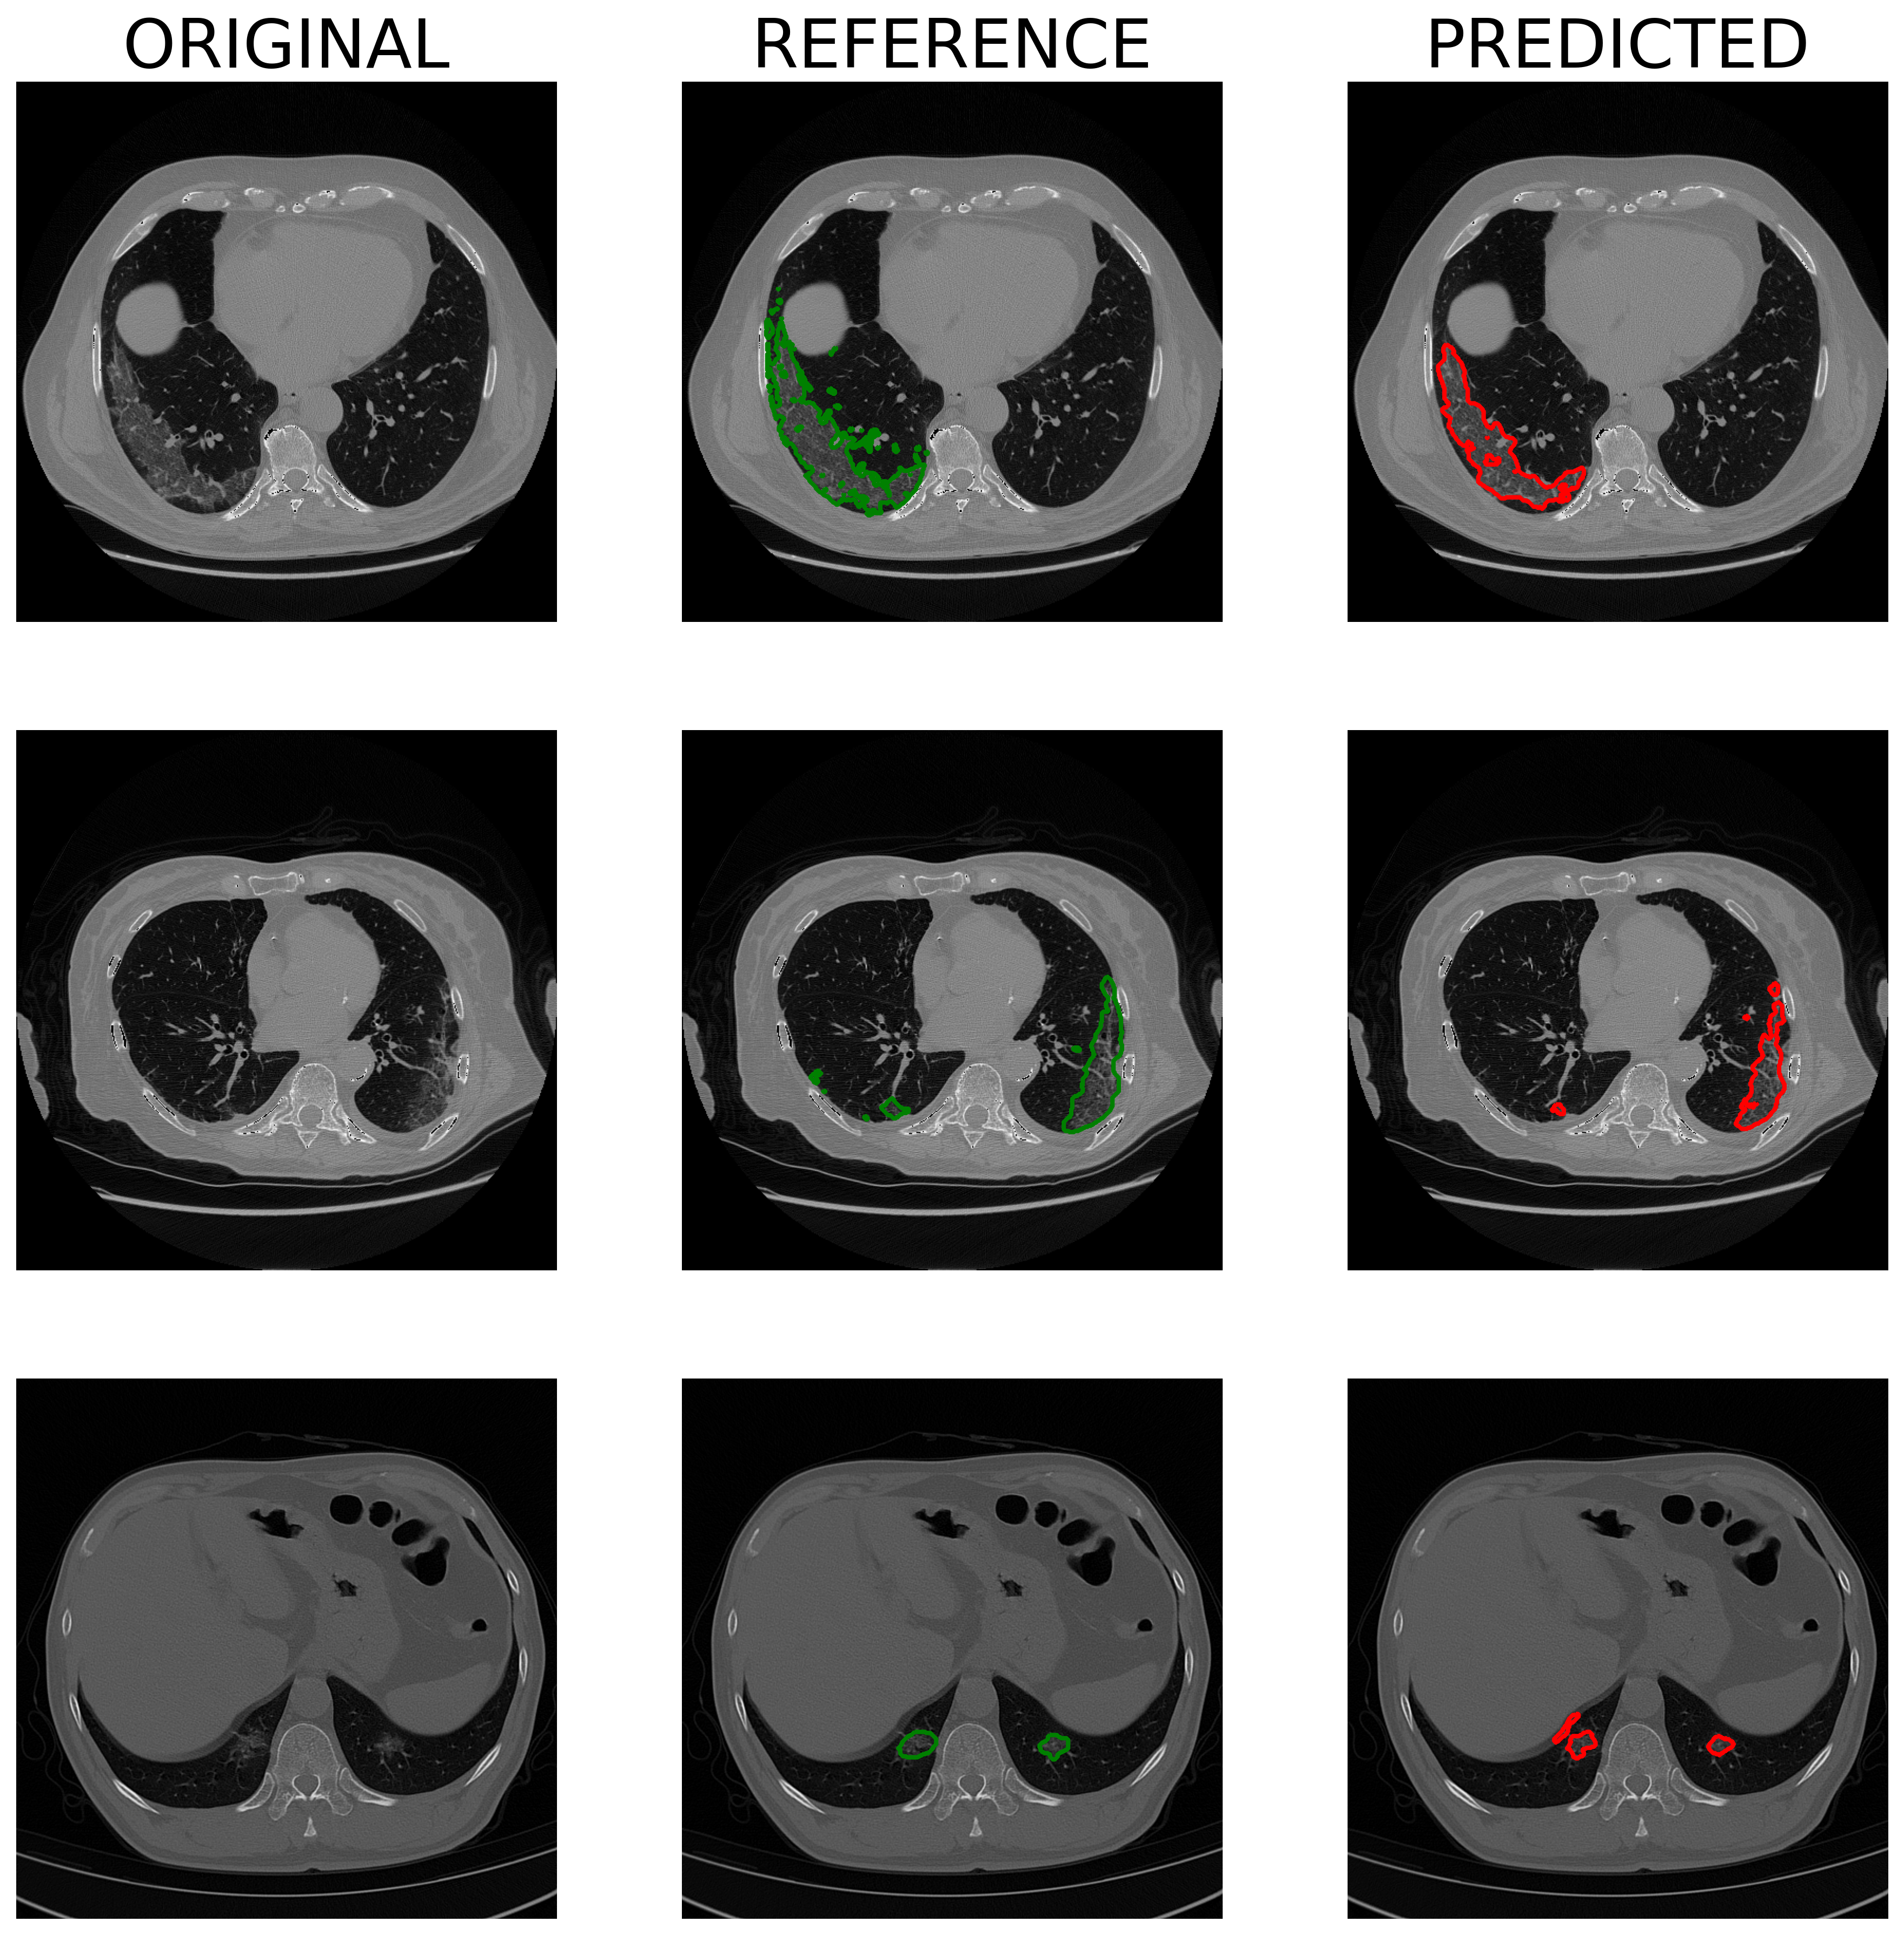
\includegraphics[width=\linewidth]{Results1.png}
		\caption{Comparison between the achieved segmentation (red) and the annotation (green). We clearly see that the GGO ans CS areas are well identified and segmentented.}\label{fig:Results}
	\end{figure}



	In \figurename\,\ref{fig:Results} I have reported a comparison between the achieved segmentation and the manual annotation as well as the original image. As we can see the lesion areas seem correctly identified. The resulting segmentation and the annotation seems to be in agreement. We can observed that the in the first case the annotation find some spots outside the main GGO area. 
	
	\begin{figure}[h!]
		\centering
			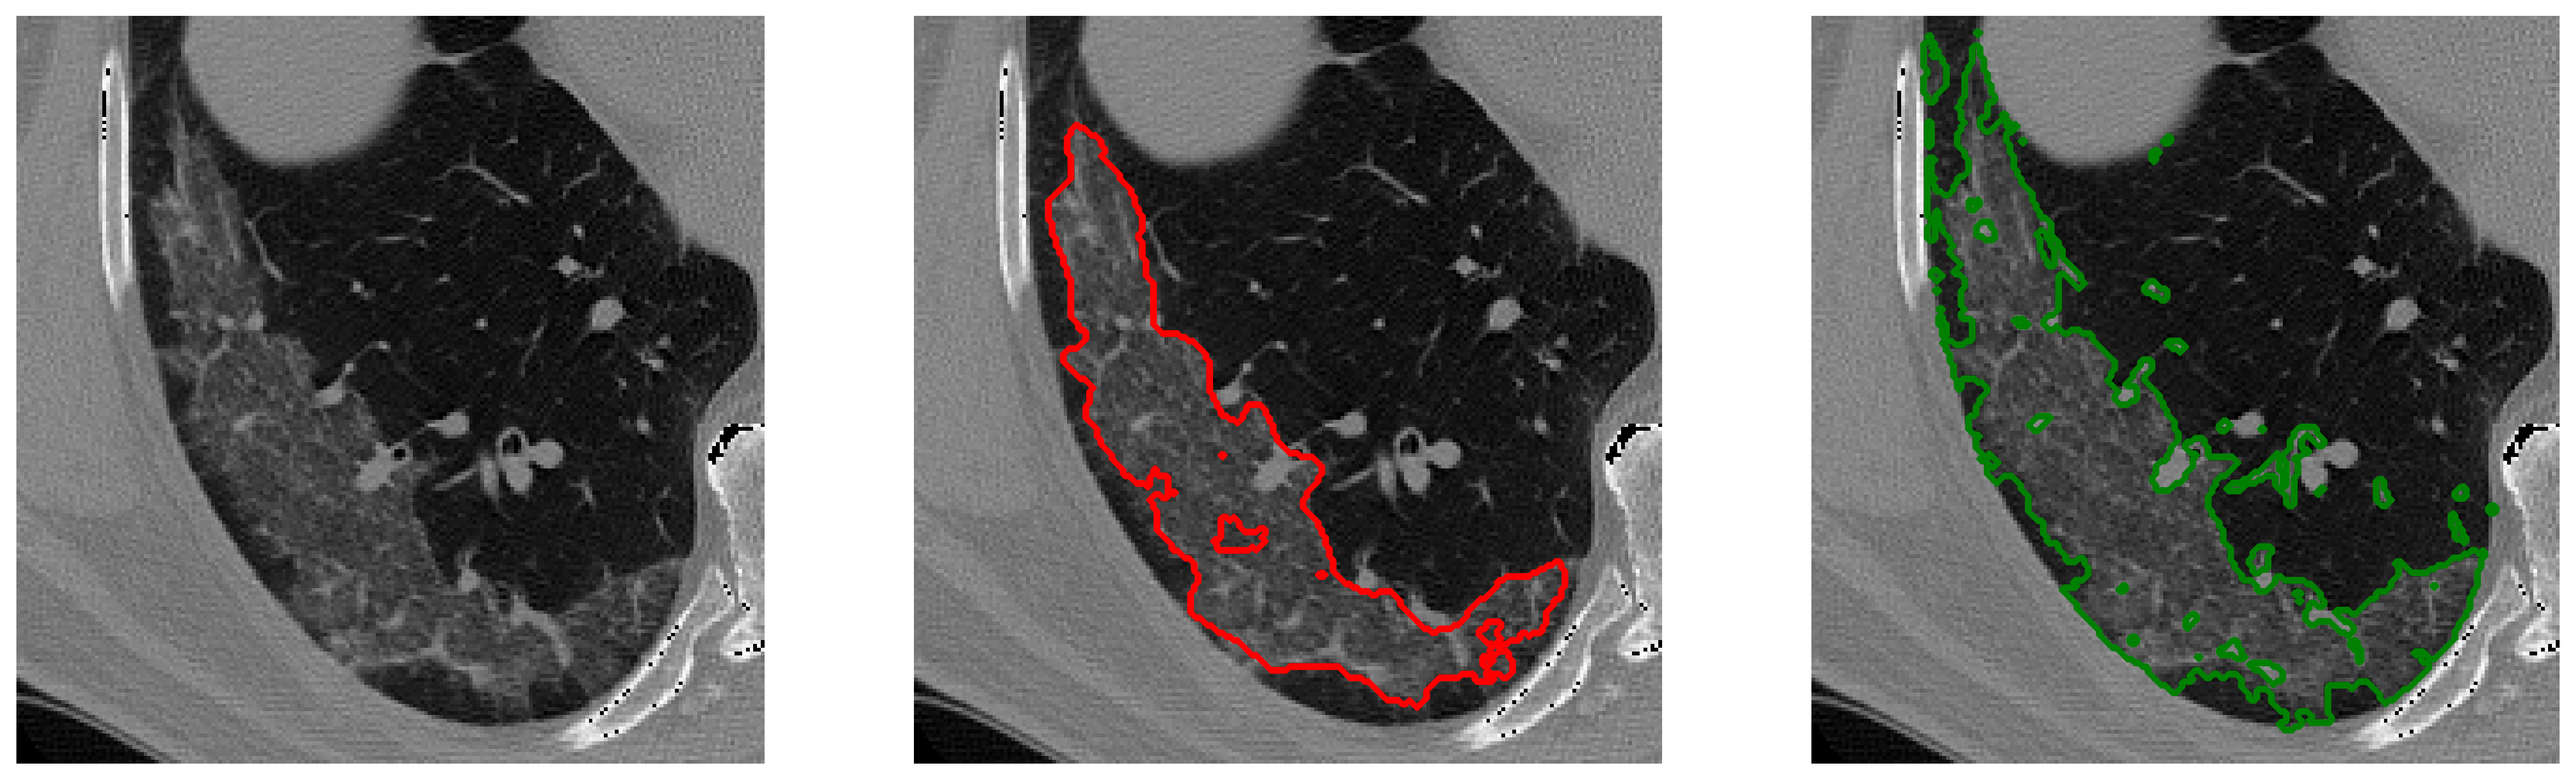
\includegraphics[scale=.37]{zoom.png}
		\caption{Focus on lesion area. From left to right we can observe the original image, the predicted lesion areas and the reference one. We can observe that the annotation  identify a larger area. The annotation identify also some spots outside the lesions which seems to be healthy tissue}\label{fig:zoom}
	\end{figure}

	In \figurename\,\ref{fig:zoom} I have provide a zoom on these interesting areas. We can see that the pipeline segmentation well identified the main opacities. We can spot that the  annotation tends to consider as GGO a larger region thn the pipeline. We can also notice that in the provided annotation also some regions that seems to be healthy are segmented.
	
		
	\begin{figure}[h!]
		
		\centering 
		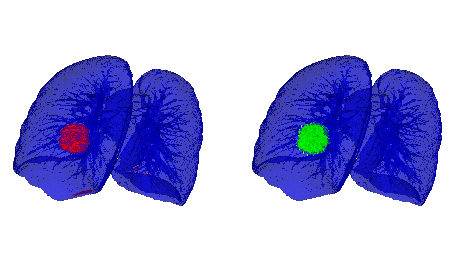
\includegraphics[scale=.4]{3Dlesion.png}
		\caption{3D representation of lesions. From left to right the manual annotation (pink) and the pipeline segmentation (green). We can observe that the segmented size of the area is different.}\label{fig:3Dlabel}		
	\end{figure}
	
	In \figurename\,\ref{fig:3Dlabel} we can see the 3D structure of the lung regions with the identified GGO and CS. In green we can observe the pipeline results; in pink the manual annotation. As we can see the two regions seem to be consistent. Again we can spot that the  annotation tends to consider a larger areas than the pipeline.
	
	I have also match results and annotation in a quantitative way. Using the $5$ ground truth (accurate and validated manual segmentations) I have matched pipeline and annotation considering sensitivity and specificity.
	Moreover, in collaboration with the Department of Diagnostic and Preventive Medicine of the Poloclinico Sant'Orsola - Malpighi, that the segmentation was submitted to five experts in order to made a blind evaluation, comparing the pipeline segmentation with annotation. 
	%In the end, as benchmark, I have segmented CT scans from healthy controls, to ensure that no lesion areas is identified. 
	
	
	
\end{document} 